\documentclass{article}

\usepackage{fancyhdr} % Required for custom headers
\usepackage{lastpage} % Required to determine the last page for the footer
\usepackage{extramarks} % Required for headers and footers
\usepackage[usenames,dvipsnames]{color} % Required for custom colors
\usepackage{graphicx} % Required to insert images
\usepackage{listings} % Required for insertion of code
\usepackage{courier} % Required for the courier font
\usepackage{lipsum} % Used for inserting dummy 'Lorem ipsum' text into the template
\usepackage{amsmath}
\usepackage{amssymb}
\usepackage{mathtools, xparse}
\usepackage{booktabs}
\usepackage{bigstrut}
\usepackage{float}
\usepackage{hyperref}
\usepackage{color}
\usepackage{algorithm}
\usepackage{caption}
\usepackage{algpseudocode}
\usepackage{multirow}


\DeclarePairedDelimiter{\norm}{\lVert}{\rVert}
\DeclarePairedDelimiter\abs{\lvert}{\rvert}%

\hypersetup{
    colorlinks   = true,    % Colours links instead of ugly boxes
    urlcolor     = red,    % Colour for external hyperlinks
    linkcolor    = red,    % Colour of internal links
    citecolor    = red      % Colour of citations
}
% Margins
\topmargin=-0.45in
\evensidemargin=0in
\oddsidemargin=0in
\textwidth=6.5in
\textheight=9.0in
\headsep=0.25in

\linespread{1.1} % Line spacing

% Set up the header and footer
\pagestyle{fancy}
\lhead{\hmwkAuthorName} % Top left header
\chead{\hmwkClass\ : \hmwkID} % Top center head
\rhead{\firstxmark} % Top right header
\lfoot{\lastxmark} % Bottom left footer
\cfoot{} % Bottom center footer
\rfoot{Page\ \thepage\ of\ \protect\pageref*{LastPage}} % Bottom right footer
\renewcommand\headrulewidth{0.4pt} % Size of the header rule
\renewcommand\footrulewidth{0.4pt} % Size of the footer rule

\setlength\parindent{0pt} % Removes all indentation from paragraphs

%----------------------------------------------------------------------------------------
%	CODE INCLUSION CONFIGURATION
%----------------------------------------------------------------------------------------

\definecolor{MyDarkGreen}{rgb}{0.0,0.4,0.0} % This is the color used for comments
\lstloadlanguages{Perl} % Load Perl syntax for listings, for a list of other languages supported see: ftp://ftp.tex.ac.uk/tex-archive/macros/latex/contrib/listings/listings.pdf
\lstset{language=Perl, % Use Perl in this example
    frame=single, % Single frame around code
    basicstyle=\small\ttfamily, % Use small true type font
    keywordstyle=[1]\color{Blue}\bf, % Perl functions bold and blue
    keywordstyle=[2]\color{Purple}, % Perl function arguments purple
    keywordstyle=[3]\color{Blue}\underbar, % Custom functions underlined and blue
    identifierstyle=, % Nothing special about identifiers                                         
    commentstyle=\usefont{T1}{pcr}{m}{sl}\color{MyDarkGreen}\small, % Comments small dark green courier font
    stringstyle=\color{Purple}, % Strings are purple
    showstringspaces=false, % Don't put marks in string spaces
    tabsize=5, % 5 spaces per tab
    %
    % Put standard Perl functions not included in the default language here
    morekeywords={rand},
    %
    % Put Perl function parameters here
    morekeywords=[2]{on, off, interp},
    %
    % Put user defined functions here
    morekeywords=[3]{test},
    %
    morecomment=[l][\color{Blue}]{...}, % Line continuation (...) like blue comment
    numbers=left, % Line numbers on left
    firstnumber=1, % Line numbers start with line 1
    numberstyle=\tiny\color{Blue}, % Line numbers are blue and small
    stepnumber=5 % Line numbers go in steps of 5
}

% Creates a new command to include a perl script, the first parameter is the filename of the script (without .pl), the second parameter is the caption
\newcommand{\perlscript}[2]{
    \begin{itemize}
        \item[]\lstinputlisting[caption=#2,label=#1]{#1.py}
    \end{itemize}
}
\newcommand{\cppscript}[1]{
    \begin{itemize}
        \item[]\lstinputlisting[]{#1}
    \end{itemize}
}

%----------------------------------------------------------------------------------------
%	DOCUMENT STRUCTURE COMMANDS
%	Skip this unless you know what you're doing
%----------------------------------------------------------------------------------------

% Header and footer for when a page split occurs within a problem environment
\newcommand{\enterProblemHeader}[1]{
    \nobreak\extramarks{#1}{#1 continued on next page\ldots}\nobreak
    \nobreak\extramarks{#1 (continued)}{#1 continued on next page\ldots}\nobreak
}

% Header and footer for when a page split occurs between problem environments
\newcommand{\exitProblemHeader}[1]{
    \nobreak\extramarks{#1 (continued)}{#1 continued on next page\ldots}\nobreak
    \nobreak\extramarks{#1}{}\nobreak
}

%\setcounter{secnumdepth}{0} % Removes default section numbers
\newcounter{homeworkProblemCounter} % Creates a counter to keep track of the number of problems

\newcommand{\homeworkProblemName}{}
\newenvironment{homeworkProblem}[1][Problem \arabic{homeworkProblemCounter}]{ % Makes a new environment called homeworkProblem which takes 1 argument (custom name) but the default is "Problem #"
    \stepcounter{homeworkProblemCounter} % Increase counter for number of problems
    \renewcommand{\homeworkProblemName}{#1} % Assign \homeworkProblemName the name of the problem
    \section{\homeworkProblemName} % Make a section in the document with the custom problem count
    \enterProblemHeader{\homeworkProblemName} % Header and footer within the environment
    }{
    \exitProblemHeader{\homeworkProblemName} % Header and footer after the environment
}

\newcommand{\problemAnswer}[1]{ % Defines the problem answer command with the content as the only argument
\noindent\framebox[\columnwidth][c]{\begin{minipage}{0.98\columnwidth}#1\end{minipage}} % Makes the box around the problem answer and puts the content inside
}

\newcommand{\homeworkSectionName}{}
\newenvironment{homeworkSection}[1]{ % New environment for sections within homework problems, takes 1 argument - the name of the section
    \renewcommand{\homeworkSectionName}{#1} % Assign \homeworkSectionName to the name of the section from the environment argument
    \subsection{\homeworkSectionName} % Make a subsection with the custom name of the subsection
    \enterProblemHeader{\homeworkProblemName\ [\homeworkSectionName]} % Header and footer within the environment
    }{
    \enterProblemHeader{\homeworkProblemName} % Header and footer after the environment
}

%----------------------------------------------------------------------------------------
%	NAME AND CLASS SECTION
%----------------------------------------------------------------------------------------

\newcommand{\hmwkID}{homework 06} % Assignment title
\newcommand{\hmwkTitle}{Matrix Condition Numbers}
\newcommand{\hmwkDueDate}{Tuesday,\ April\ 11,\ 2017} % Due date
\newcommand{\hmwkClass}{Numerical Analysis} % Course/class
\newcommand{\hmwkClassTime}{10:30am} % Class/lecture time
\newcommand{\hmwkClassInstructor}{Jones} % Teacher/lecturer
\newcommand{\hmwkAuthorName}{102061149 Fu-En Wang} % Your name

%----------------------------------------------------------------------------------------
%	TITLE PAGE
%----------------------------------------------------------------------------------------

\title{
    \vspace{2in}
    \textmd{\textbf{\hmwkClass}}\\
    \textmd{\textbf{\hmwkID: \hmwkTitle}} \\
    \normalsize\vspace{0.1in}\small{Due\ on\ \hmwkDueDate}\\
    \vspace{3in}
}

\author{\textbf{\hmwkAuthorName}}
\date{} % Insert date here if you want it to appear below your name

%----------------------------------------------------------------------------------------

\begin{document}
\maketitle
\newpage

\section{Introduction}
In this homework, we will implement the Power Method algorithm to find certain eigenvalues of a given matrix $A$.
\subsection{Termination Condition}
To calculate error of each iteration, we will use four kind of error fomula:
\begin{enumerate}
    \item $\epsilon_1 = \abs{{V^{(k+1)} - V^{k}}}$
    \item $\epsilon_2 = {\norm{q^{(k+1)} - q^k}}_2$
    \item $\epsilon_3 = \norm{r^{(k+1)}}$
    \item $\epsilon_4 = \frac{\norm{r^{(k+1)}}}{\abs{(W^k)^Tq^k}}$
\end{enumerate}
where $r^k = Aq^k - V^kq^k$ and $W^k = \frac{(q^k)^TA}{\norm{(q^k)^TA}_2}$. In this project, we need to use the four error to 
test Power Method and find out which error we prefer.

\subsection{Power Method}
We will implement three Power Method algorithm to find eigenvalue.
\begin{enumerate}
    \item \textbf{Power Method}(to find largest eigenvalue).
    \item \textbf{Inverse Power Method}(to find smallest eigenvalue).
    \item \textbf{Inverse Power Method with Shift}(to find eigenvalue closest to $\omega$).
\end{enumerate}

\subsection{Condition Numbers}
Condition Numbers is defined as
$$
    k = \frac{\lambda_1}{\lambda_n}
$$
We need to find the condition numbers of the following resistor network.
\begin{enumerate}
    \item $2 \times 2$ resistor network
    \item $4 \times 4$ resistor network
    \item $10 \times 10$ resistor network
    \item $20 \times 20$ resistor network
    \item $40 \times 40$ resistor network
    \item $50 \times 50$ resistor network
\end{enumerate}
\newpage

\section{Implementation}
\begin{algorithm}[H]
    \caption{\textbf{Power Method}}
    \begin{algorithmic}
        \For{each k $\in$ \{1, ..., maxIter\}}
            \State $q^{(k+1)} = \frac{Aq^k}{\norm{Aq^k}_2}$
            \State $V^{(k+1)} = (q^k)^TAq^k$
            \If{$error < tol$}
                \State break
            \EndIf
        \EndFor
    \end{algorithmic}
\end{algorithm}
\begin{algorithm}[H]
    \caption{\textbf{Inverse Power Method}}
    \begin{algorithmic}
        \For{each k $\in$ \{1, ..., maxIter\}}
            \State $Az^k = q^{(k-1)}$
            \State $q^k = \frac{z^k}{\norm{z^k}_2}$
            \State $V^k = (q^k)^TAq^k$
            \If{$error < tol$}
                \State break
            \EndIf
        \EndFor
    \end{algorithmic}
\end{algorithm}
\begin{algorithm}[H]
    \caption{\textbf{Inverse Power Method with Shift}}
    \begin{algorithmic}
        \For{each k $\in$ \{1, ..., maxIter\}}
            \State $(A - {\omega}I)z^k = q^{(k-1)}$
            \State $q^k = \frac{z^k}{\norm{z^k}_2}$
            \State $V^k = (q^k)^TAq^k$
            \If{$error < tol$}
                \State break
            \EndIf
        \EndFor
    \end{algorithmic}
\end{algorithm}
\subsection{Complexity}
\label{sec:complexity}
For each iteration of the three Power Method, the most time-consuming part is Matrix x Vector, which is a {\boldmath$O(n^2)$} problem. 
However, because I use LU Decomposition for Inverse Power Method and Inverse Power Method with Shift, so their overall runtime should be 
influenced by {\boldmath$O(n^3)$}.


\section{Discussion of Termination Condition}
\label{sec:part1}
In this section, we will discuss which termination condition is the best. Table \ref{tab:termination condition} shows average iteration
time of a 20 x 20 resostor network.
\begin{table}[H]
    \begin{center}
        \begin{tabular}{|c|c|c|c|c|}
            \hline
                & $\epsilon_1$ & $\epsilon_2$ & $\epsilon_3$ & $\epsilon_4$ \\ \hline
            \# of iter & 299 & 795 & 683 & 683 \\ \hline
            $\lambda$ & 0.0795492 & 0.0795492 & 0.0795492 & 0.0795492 \\ \hline
            Runtime & 0.073175 & 0.163965 & 0.149694 & 0.303234 \\ \hline
            iter\_avg & 2.45E-04 & 2.06E-04 & 2.19E-04 & 4.44E-04 \\ \hline
        \end{tabular}
    \end{center}
    \caption{Average iteration time of 20 x 20 resistor network}
    \label{tab:termination condition}
\end{table}
In Table \ref{tab:termination condition}, $\epsilon_4$ has the largest iter\_avg, while $\epsilon_2$ has the smallest. For more detailed
observation, I plot the error vs iter as shown in Figure \ref{fig:termination condition}.
\begin{figure}[H]
    \centering
    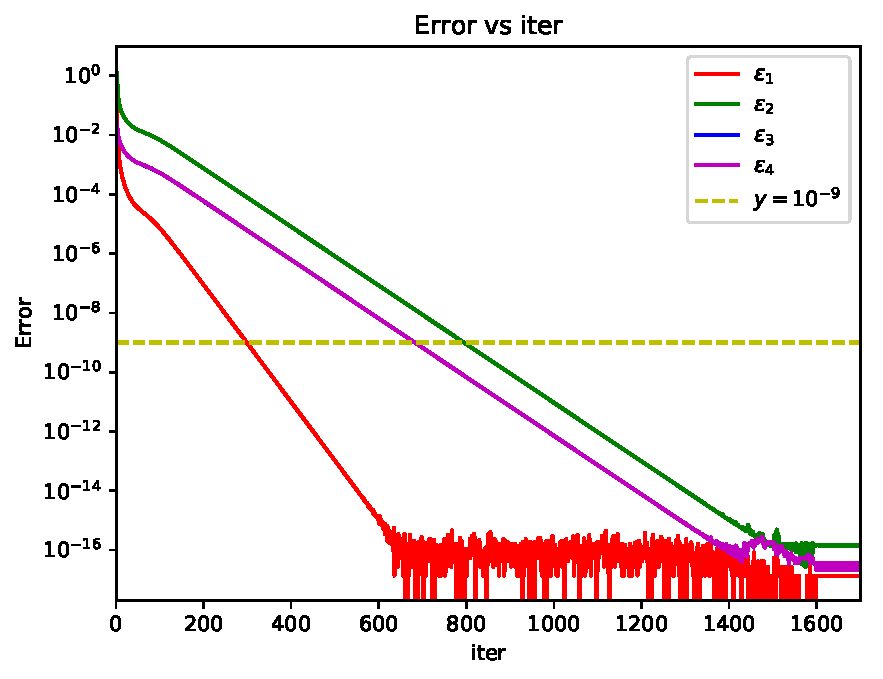
\includegraphics[width=0.7\textwidth]{src/error_1234.pdf}
    \caption{Error vs iter of 20 x 20 resistor network}
    \label{fig:termination condition}
\end{figure}
In Figure \ref{fig:termination condition}, $\epsilon_3$ and $\epsilon_4$ almost overlap together and we can find that $\epsilon_1$ has the smallest 
number of iteration to converge. In addition, because the purpose of Power Method is to find the eigenvalue, so I think we just need to check 
the convergence of lambda. As a result, I think \textbf{{\boldmath$\epsilon_1$} is the best}.

\section{Discussion of Power Method}
In this section, we will determine the condition number of several resistor network and discuss the complexity of the three Power Method. 
Table \ref{tab:pwr}, \ref{tab:ipwr} and \ref{tab:ipwrsht} show the detailed result of experiment with different resistor number.
\begin{table}[H]
    \begin{center}
        \begin{tabular}{|c|c|c|c|c|c|c|}
            \hline
            resistor num & 2 & 4 & 10 & 20 & 40 & 50 \\ \hline
            N & 9 & 25 & 121 & 441 & 1681 & 2601 \\ \hline
            \# of iter & 27 & 21 & 91 & 299 & 984 & 1439 \\ \hline
            runtime(s) & 3.70E-05 & 7.10E-05 & 1.68E-03 & 7.04E-02 & 2.98E+00 & 1.04E+01 \\ \hline
            iter\_avg(s) & 1.37E-06 & 3.38E-06 & 1.84E-05 & 2.36E-04 & 3.03E-03 & 7.22E-03 \\ \hline
            $\lambda$ & 0.00523607 & 0.0142445 & 0.0391638 & 0.0795492 & 0.159765 & 0.19981 \\ \hline
        \end{tabular}
    \end{center}
    \caption{Result of Power Method}
    \label{tab:pwr}
\end{table}
\begin{table}[H]
    \begin{center}
        \begin{tabular}{|c|c|c|c|c|c|c|}
            \hline
            resistor num & 2 & 4 & 10 & 20 & 40 & 50 \\ \hline
            N & 9 & 25 & 121 & 441 & 1681 & 2601 \\ \hline
            \# of iter & 11 & 8 & 5 & 4 & 4 & 3 \\ \hline
            runtime(s) & 2.40E-05 & 0.000153 & 0.004976 & 0.211479 & 12.4805 & 42.3624 \\ \hline
            iter\_avg(s) & 1.82E-06 & 6.00E-06 & 1.15E-04 & 1.46E-03 & 2.14E-02 & 5.91E-02 \\ \hline
            $\lambda$ & 0.000763932 & 0.000390179 & 0.000129496 & 5.42E-05 & 2.28E-05 & 1.73E-05 \\ \hline
        \end{tabular}
    \end{center}
    \caption{Result of Inverse Power Method}
    \label{tab:ipwr}
\end{table}
\begin{table}[H]
    \begin{center}
        \begin{tabular}{|c|c|c|c|c|c|c|}
            \hline
            resistor num & 2 & 4 & 10 & 20 & 40 & 50 \\ \hline
            N & 9 & 25 & 121 & 441 & 1681 & 2601 \\ \hline
            \# of iter & 11 & 7 & 5 & 3 & 4 & 4 \\ \hline
            runtime(s) & 3.80E-05 & 1.59E-04 & 5.19E-03 & 2.17E-01 & 1.23E+01 & 4.31E+01 \\ \hline
            iter\_avg(s) & 2.00E-06 & 5.71E-06 & 1.15E-04 & 1.53E-03 & 2.54E-02 & 5.65E-02 \\ \hline
            $\lambda$ & 0.000763932 & 0.000390179 & 0.000129496 & 5.42E-05 & 2.28E-05 & 1.73E-05 \\ \hline
        \end{tabular}
    \end{center}
    \caption{Result of Inverse Power Method with Shift(mu = 5E-05)}
    \label{tab:ipwrsht}
\end{table}
Because Condition Number is $\frac{\lambda_1}{\lambda_n}$, so we can get Condition Number of the 6 resistor networks from the tables above,
as shown in Table \ref{tab:condition number}.
\begin{table}[htbp]
    \begin{center}
        \begin{tabular}{|c|c|c|c|c|c|c|}
            \hline
            resistor num & 2 & 4 & 10 & 20 & 40 & 50 \\ \hline
            N & 9 & 25 & 121 & 441 & 1681 & 2601 \\ \hline
            condition num & 6.8541 & 36.5077 & 302.432 & 1467.21 & 7016.84 & 11574.3 \\ \hline
        \end{tabular}
    \end{center}
    \caption{Condition Number of the 6 resistor networks}
    \label{tab:condition number}
\end{table}

\subsection{Complexity}
From Table \ref{tab:pwr}, \ref{tab:ipwr} and \ref{tab:ipwrsht}, we can plot \textbf{iter\_avg vs N} and \textbf{overall runtime vs N} as shown in 
Figure \ref{fig:iter_avg vs N} and \ref{fig:runtime vs N}.
\begin{figure}[H]
    \centering
    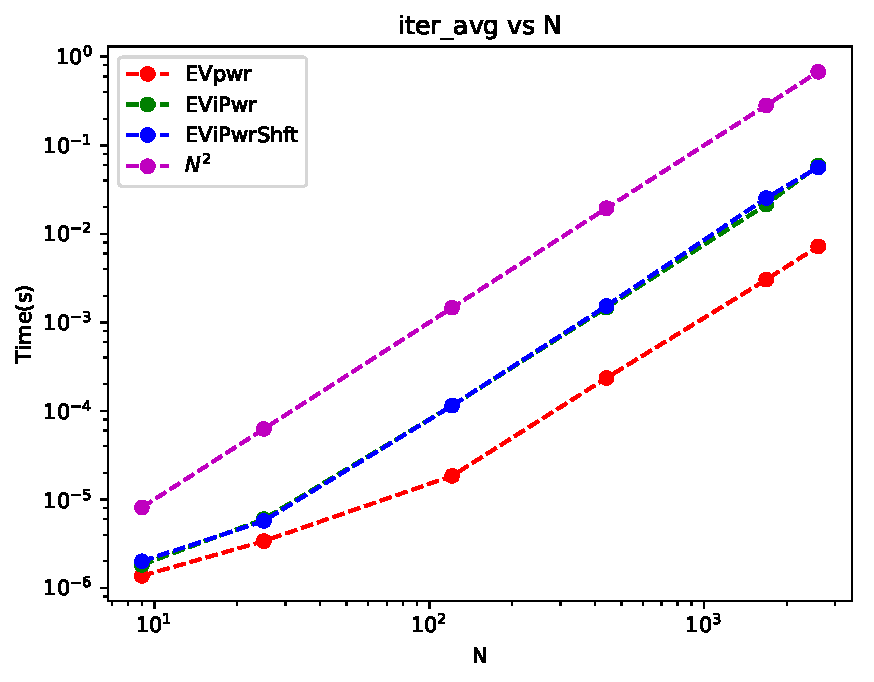
\includegraphics[width=0.7\textwidth]{src/iter_avg.pdf}
    \caption{iter\_avg vs N}
    \label{fig:iter_avg vs N}
\end{figure}
\begin{figure}[H]
    \centering
    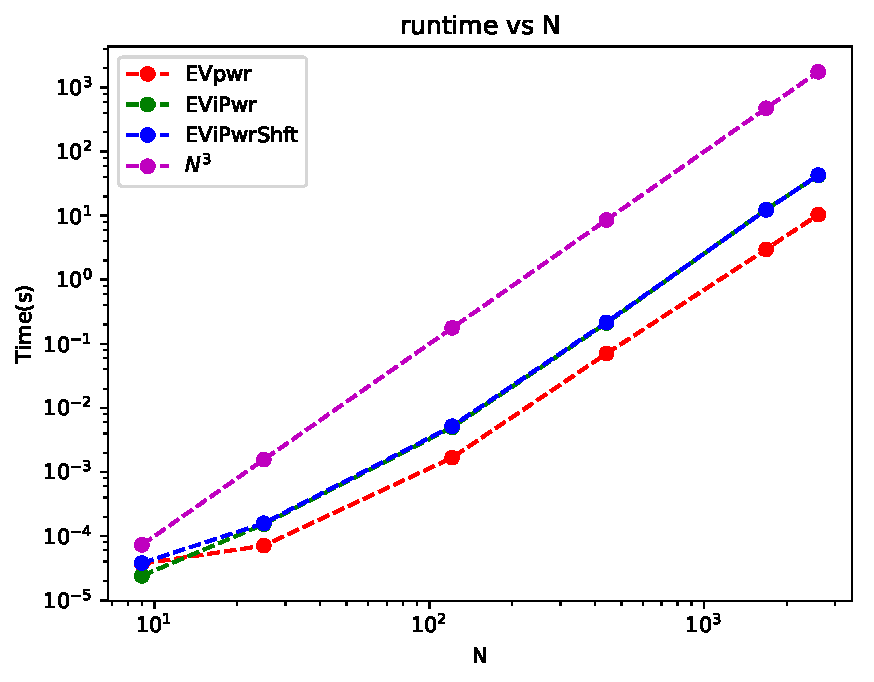
\includegraphics[width=0.7\textwidth]{src/runtime.pdf}
    \caption{runtime vs N}
    \label{fig:runtime vs N}
\end{figure}
In Figure \ref{fig:iter_avg vs N} and \ref{fig:runtime vs N}, EViPwr and EViPwrShft almost overlap together because they have almost same speed.
From Figure \ref{fig:iter_avg vs N}, we can find that the slope of each iteration of the three Power Method is same as $N^2$, which means
each iteration is a $O(n^2)$ problem. From Figure \ref{fig:runtime vs N}, we can find that the slope of runtime of Inverse Power Method and
Inverse Power Method with Shift is almost same as $N^3$, this is because the overall runtime will be affected by \textbf{LU Decomposition}, 
which is $O(n^3)$ problem. For EVpwr, it seems that EVpwr also have $N^3$ slope, but I think this will vary from our initial guess. If
we have a initial guess close to answer then the iteration number will drop and change the slope.

\end{document}













